\scanpage{71}
\uline{Lemme 4}

% slanted
\margin{\uline{NB} Il y a une version plus faible de A), où $\dot U=C$ (sans $I$), qui n'est pas formellement contenue ds A).}

A) Soit $U$ une partie ouverte bornée
de $\mathbb{C}$, dont la frontière est \inserted{réunion de} une
courbe de Jordan \deleted{rectifiable. Alors
il existe une \unsure{fonction,|fonction} continue
$f:\mathbb{D}\longrightarrow$}
$C$, et d'un \deleted{homéomorphisme} intervalle
topologique $I$ tel que
$I\cap C=\{b\}$, \deleted{\unsure{et}} (alors $I\setminus\{b\}$ est
contenu dans la comp. connexe
bornée $V$ de $\mathbb{C}\setminus C$, et $b$
est une extrémité de $I$, \inserted{notons $U=V\setminus I'$, où $I'=I\setminus\{b\}$}). \deleted{Soit} On
suppose de plus que $C$ et $I$ soient rectifiables.
Soit $a$ l'autre extrémité de $I$. Alors il
existe une fonction \deleted{continue} $f:\mathbb{D}\longrightarrow\mathbb{C}$
telle que

\figure{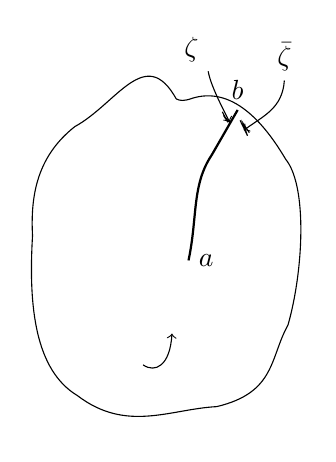
\begin{tikzpicture}[x=.78cm,y=.78cm]
\draw (0,2.1) .. controls (-.5,3) and (-.97,2.02) .. (-1.65,1.65) .. controls (-2.3,1.14) and (-2.37,.46) .. (-2.34,-.13) .. controls (-2.41,-1.30) and (-2.29,-2.32) .. (-1.61,-2.73) .. controls (-.81,-3.34) and (-.10,-2.95) .. (.66,-2.91) .. controls (1.62,-2.68) and (1.52,-2.12) .. (1.82,-1.58) .. controls (2.07,-.70) and (2.14,.68) .. (1.78,1.12) .. controls (1.35,1.85) and (.84,2.29) .. (.26,2.11) .. controls (.12,2.06) and (.06,2.07) .. (0,2.1);
\draw[thick] (.2,-.53) node[right]{$a$} .. controls (.35,.18) and (.25,.7) .. (.58,1.19) -- (1,1.92) node[above]{$b$};
\draw[->] (.52,2.55) node[above left]{$\zeta$} .. controls (.56,2.32) and (.75,1.96) .. (.87,1.72);
\draw[->] (1.76,2.40) node[above]{$\bar\zeta$} .. controls (1.73,1.94) and (1.41,1.82) .. (1.10,1.59);
\draw (.75,1.89) -- (.84,1.72) -- (.77,1.83) -- (.88,1.71);
\draw (1.04,1.75) -- (1.16,1.50) -- (1.09,1.70) -- (1.19,1.55);
\draw[->] (-.54,-2.23) .. controls (-.34,-2.37) and (-.10,-2.24) .. (-.07,-1.72);
\end{tikzpicture}}

1) $f$ est continue, et induit une \deleted{ho} bijection
(voire un homéo !) $\mathring{\mathbb{D}}\xrightarrow{\sim}U$.

2) $f(\zeta)=f(\bar\zeta)=b$, et $f$ induit une bijection
(voire un homéo) $\deleted{\alpha}\inserted{\alpha\setminus\{\zeta\bar\zeta\}}\xrightarrow{\sim} C\setminus\{b\}$.
(NB $\zeta=\exp 2i\pi/3$, et $\alpha,\beta,\bar\beta$ sont les trois
arcs sur $\partial\mathbb{D}$ déterminés par $1,\zeta,\bar\zeta$).

\figure{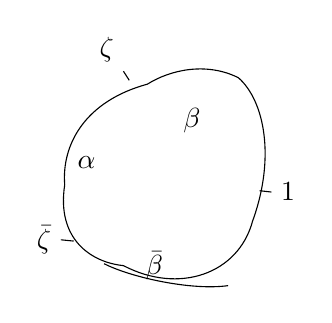
\begin{tikzpicture}[scale=.82]
\draw (1.1,1.4) .. controls (.6,1.65) and (.04,1.52) .. (-.31,1.30) .. controls (-1.27,1.04) and (-1.64,.37) .. (-1.59,-.26) .. controls (-1.72,-1.10) and (-1.18,-1.46) .. (-.68,-1.51) .. controls (.18,-1.96) and (1.1,-1.64) .. (1.32,-.82) .. controls (1.68,.17) and (1.50,1.05) .. (1.1,1.4);
\draw (-.59,1.36)--(-.68,1.50) node[above left]{$\zeta$};
\draw (-1.45,-1.13)--(-1.65,-1.11) node[left]{$\bar\zeta$};
\draw (1.43,-.35)--(1.61,-.37) node[right]{$1$};
\node at (-1.25,.09){$\alpha$};\node at (.38,.74){$\beta$};\node at (-.20,-1.51){$\bar\beta$};
\draw (-.98,-1.48) .. controls (-.57,-1.69) and (.37,-1.90) .. (.94,-1.82);
\end{tikzpicture}}

3) $f\mid\beta$ et $f\mid\bar\beta$ induisent des bijections de
$\beta$ et $\bar\beta$ sur $I$). NB a) b) c) peuvent
s'exprimer en disant que $f$ induit un
\deleted{\unsure{isom}} \inserted{homéo} de $\mathbb{D}$ sur le découpé de $\bar U=\bar V$
suivant $I$ (ou sur $I\cup C=\dot U$).

4) $f\mid\mathring{\mathbb{D}}$ est holomorphe.
% archive sheet number: 73
